\lstinputlisting[firstline=194,lastline=199]{StreamsUndMengen.rkt}
Konvertierung Liste xs in eine Menge gleicher Elemente.\\
\begin{minipage}{0.45\textwidth}
	\begin{tikzpicture}
	\draw[black,solid] (0,0)--(0,1);
	\draw[black,solid] (0,0)--(1,0);
	\draw[black,solid] (0,1)--(1,1);
	\draw[black,solid] (1,1)--(1,0);
	\draw[black,solid] (0.5,1)--(0.5,0);
	\node () at (0.25,0.5) {$x_1$};
	\draw[black,solid] (0.75,0.5)--(1.5,-0.75);
	\draw[black,solid] (1.5,-0.75)--(1.5,-1.75);
	\draw[black,solid] (1.5,-0.75)--(2.5,-0.75);
	\draw[black,solid] (1.5,-1.75)--(2.5,-1.75);
	\draw[black,solid] (2.5,-1.75)--(2.5,-0.75);
	\draw[black,solid] (2.0,-1.75)--(2.0,-0.75);
	\node () at (1.75,-1.25) {$x_2$};
	\draw[black,dashed] (2.25,-1.25)--(3,-2.5);
	\draw (3,-2.5)rectangle(4,-3.5);
	\draw[black,solid] (3.5,-2.5)--(3.5,-3.5);
	\node () at (3.85,-3.5) {\begin{rotate}{90}
		\lstinline!empty!
		\end{rotate}};
	\node () at (3.25,-3) {$x_n$};
	\end{tikzpicture}
\end{minipage}%
\begin{minipage}{0.15\textwidth}
	\lstinline|(fold empty-set set-insert xs)|\eval 
\end{minipage}%
\begin{minipage}{0.4\textwidth}
	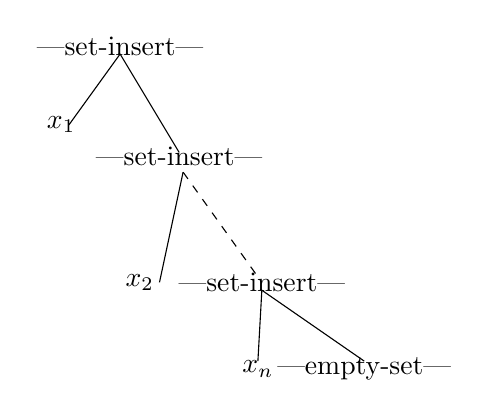
\begin{tikzpicture}
	\node () at (0,-0.4) {$x_1$};
	\draw[black,solid] (0.75,0.5)--(1.5,-0.75);
	\draw[black,solid] (0.75,0.5)--(0.1,-0.4);
	\node () at (0.75,0.6) {\lstinline|set-insert|};
	\node () at (1.5,-0.8) {\lstinline|set-insert|};
	\draw[black,solid] (1.55,-1)--(1.25,-2.4);
	\node () at (1,-2.4) {$x_2$};
	\draw[black,dashed] (1.55,-1)--(2.55,-2.4);
	\node () at (2.55,-2.4) {\lstinline|set-insert|};
	\draw[black,solid] (2.55,-2.5)--(3.85,-3.4);
	\draw[black,solid] (2.55,-2.5)--(2.5,-3.4);
	\node () at (3.85,-3.5) {\lstinline|empty-set|};
	\node () at (2.5,-3.5) {$x_n$};
	\end{tikzpicture}
\end{minipage}
\rackett{Listen zu Mengen Konvertierung }{Konvertiert eine Liste zu einer Menge}{StreamsUndMengen}{56}{65}
Vereinigung: $\chi_{S \cup T}(x) = \chi_S(x) \lor \chi_T(x)$.\\
Weitere Mengenoperationen analog:
\rackett{Mengenoperationen}{Mengenoperationen $\setminus,\,\cup,\,\cap,\,\triangle $}{StreamsUndMengen}{67}{98}
Charakteristische Funktion zur Repräsentation Mengen:
\begin{enumerate}[(1)]
\item Performance: \lstinline|set-member| hat lineare Laufzeit bei mit \lstinline|set-insert| konstruierte Mengen (wie Liste!)
\item Vorteile:
\subitem+ unendliche Mengen darstellbar
\subitem+ Mengenoperationen in konstanter Zeit durchführbar
\item Nachteile
\subitem- Elemente sind nicht auf zählbar
\end{enumerate}
\emph{Streams}\lstinline|(stream-of %a)|:unendliche Ströme von Elementen x, mit Signatur \%a
Ein Stream ist ein Paar:\\
\begin{figure}[h!]
\centering
\begin{tikzpicture}
\node () at (-1.7,0.5) {Streamhead};
\draw[->] (-0.5,0.5)--(-0.1,0.5);
\draw (0,0)rectangle(1,1);
\node () at (0.5,0.5) {$x_1$};
\node () at (0.3,-0.2) {\%a};
\draw (1,1)rectangle(4,0);
\node () at (2.5,0.5) {\lstinline|tail|};
\node () at (3,-0.2) {\lstinline|(->(stream-of %a))|};
\end{tikzpicture}
\end{figure}
-Erst eine Ausführung des Tails (\emph{\lstinline|force|}) erzeugt nächstes Stream-Element (faher auch \emph{lazylist}).\\
\begin{figure}[h!]
\centering
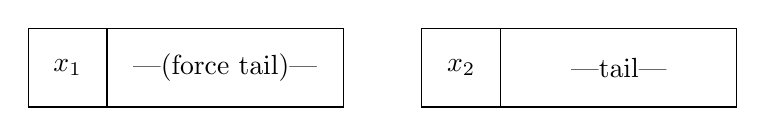
\begin{tikzpicture}
\draw (0,0)rectangle(1,1);
\node () at (0.5,0.5) {$x_1$};
\draw (1,1)rectangle(4,0);
\node () at (2.5,0.5) {\lstinline|(force tail)|};
\draw (5,0)rectangle(6,1);
\node () at (4.6,0.5) {\eval};
\node () at (5.5,0.5) {$x_2$};
\draw (6,1)rectangle(9,0);
\node () at (7.5,0.5) {\lstinline|tail|};
\end{tikzpicture}
\end{figure}
Vergleich:\\
\begin{minipage}{0.5\textwidth}
	\begin{tikzpicture}
	\draw[black,solid] (0,0)--(0,1);
	\draw[black,solid] (0,0)--(1,0);
	\draw[black,solid] (0,1)--(1,1);
	\draw[black,solid] (1,1)--(1,0);
	\draw[black,solid] (0.5,1)--(0.5,0);
	\node () at (0.25,0.5) {$x_1$};
	\draw[black,solid] (0.75,0.5)--(1.5,-0.75);
	\draw[black,solid] (1.5,-0.75)--(1.5,-1.75);
	\draw[black,solid] (1.5,-0.75)--(2.5,-0.75);
	\draw[black,solid] (1.5,-1.75)--(2.5,-1.75);
	\draw[black,solid] (2.5,-1.75)--(2.5,-0.75);
	\draw[black,solid] (2.0,-1.75)--(2.0,-0.75);
	\node () at (1.75,-1.25) {$x_2$};
	\draw[black,dashed] (2.25,-1.25)--(3,-2.5);
	\draw (3,-2.5)rectangle(4,-3.5);
	\draw[black,solid] (3.5,-2.5)--(3.5,-3.5);
	\node () at (3.85,-3.5) {\begin{rotate}{90}
		\lstinline!empty!
		\end{rotate}};
	\node () at (3.25,-3) {$x_n$};
	\end{tikzpicture}
\end{minipage}
\begin{minipage}{0.5\textwidth}
	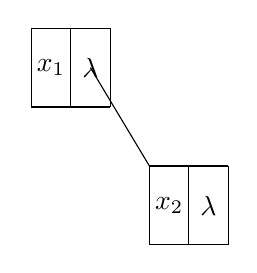
\begin{tikzpicture}
	\draw[black,solid] (0,0)--(0,1);
	\draw[black,solid] (0,0)--(1,0);
	\draw[black,solid] (0,1)--(1,1);
	\draw[black,solid] (1,1)--(1,0);
	\draw[black,solid] (0.5,1)--(0.5,0);
	\node () at (0.25,0.5) {$x_1$};
	\node () at (0.75,0.5) {$\lambda$};
	\draw[black,solid] (0.75,0.5)--(1.5,-0.75);
	\draw[black,solid] (1.5,-0.75)--(1.5,-1.75);
	\draw[black,solid] (1.5,-0.75)--(2.5,-0.75);
	\draw[black,solid] (1.5,-1.75)--(2.5,-1.75);
	\draw[black,solid] (2.5,-1.75)--(2.5,-0.75);
	\draw[black,solid] (2.0,-1.75)--(2.0,-0.75);
	\node () at (1.75,-1.25) {$x_2$};
	\node () at (2.25,-1.25) {$\lambda$};
	\end{tikzpicture}
\end{minipage}
Verzögerte Auswertung eines Ausdrucks (\emph{delayed Evaluation}):
\begin{enumerate}[-]
\item 
\lstinline|(delay e)|: Verzögere die Auswertung des Ausdruckes e und liefere ''Versprechen'' (\lstinline|promise|) e bei Bedarf später auswerten zu können.\\
\lstinline|(delay e)| $\equiv$ \lstinline[mathescape]|(lambda ()$\underset{\substack{\uparrow\\\t{nicht}\\\t{ausgewertet}}}{\t{e}}$)|\\
\lstinline|(force p)| Erzwinge Auswertung des \lstinline|promise|. p liefert Wert zurück
\end{enumerate}
\begin{lstlisting}
(: force ((-> %a)->%a))
(define force
  (lambda (p)
    (p)))
\end{lstlisting}
\rackett{Implementation von Streams}{Streams}{StreamsUndMengen}{101}{190}